\documentclass[a4paper]{ctexart}
\usepackage[top=2.3cm,bottom=2cm,left=1.7cm,right=1.7cm]{geometry} 
\usepackage{amsmath} 
\usepackage{booktabs}
\usepackage{amsthm}
\usepackage{longtable} 
\usepackage{graphicx}
\usepackage{subfigure}
\usepackage{caption}
\usepackage{fontspec}
\usepackage{titlesec}
\usepackage{fancyhdr}
\def\degree{$^{\circ}$}
\def\mm{\mathrm{mm}}
\def\cm{\mathrm{cm}}
\def\nm{\mathrm{nm}}
\def\kpa{\mathrm{kpa}}
\def\V{\mathrm{V}}
\def\m{\mathrm{m}}
\def\g{\mathrm{g}}
\def\Pa{\mathrm{Pa}}
\title{\textbf{测定金属的杨氏模量}}
\author{王崇斌 1800011716}
\date{}
\makeatletter %使\section中的内容左对齐
\renewcommand{\section}{\@startsection{section}{1}{0mm}
	{-\baselineskip}{0.5\baselineskip}{\bf\leftline}}
\makeatother
\begin{document}
	\pagestyle{fancy}
	\lhead{普通物理实验报告} 
	\chead{}
	\rhead{}
	\maketitle
	\thispagestyle{fancy}
	\section{\large{数据及处理}}
	\subsection{CCD成像系统测定杨氏模量}
	\subsubsection{实验数据记录}
	\begin{table}[htbp]
		\centering
		\caption{单个砝码质量的测量数据表}
		\begin{tabular}{cccccc}
			\toprule[1.5pt]
			单个砝码质量$m_{i0}(\g)$ & 200.03 & 200.10 & 199.83 & 199.92 & 199.99 \\
			\midrule
			 & 199.84 & 200.30 & 199.72 & 200.43 & \\
			 \bottomrule[1.5pt]
		\end{tabular}
		\label{m_data_1}
	\end{table}
	\par 
	表 1 中的数据是按照实验中向砝码托上加砝码的顺序测出的质量。由天平的分度值可以看出,
	质量测量的相对不确定度很小,我们可以认为质量测量是准确的,在线性回归求杨氏模量时将质量作为自变量。\\
	\begin{table}[htbp]
		\centering
		\caption{测量金属丝受外力拉伸后伸展变化数据表}
		\begin{tabular}{ccccc}
			\toprule[1.5pt]
			$i$ & $m_{i}(\g)$ & $r_{i}(\cm)$ & $r_{i}^{'}(\cm)$ & $\bar{r}_{i}(\cm)$\\
			\midrule
			0 & 0       & 0.415 & 0.411 & 0.413 \\
			1 & 200.03  & 0.402 & 0.400 & 0.401 \\
			2 & 400.13  & 0.388 & 0.389 & 0.3885 \\
			3 & 599.96  & 0.376 & 0.376 & 0.376 \\
			4 & 799.88  & 0.364 & 0.366 & 0.365 \\
			5 & 999.87  & 0.353 & 0.354 & 0.3535 \\
			6 & 1199.71 & 0.341 & 0.342 & 0.3415 \\
			7 & 1400.01 & 0.330 & 0.330 & 0.330 \\
			8 & 1599.73 & 0.318 & 0.318 & 0.318 \\
			9 & 1800.16 & 0.308 & 0.307 & 0.3075\\
			\bottomrule[1.5pt]
		\end{tabular}
	\end{table}
	\par 
	测量金属丝伸长量的显微镜刻线板的允差为$e = 0.05 \; \mm$
	\par 
	金属丝的长度$L=80.10\cm$,木尺的允差为$0.1\cm$
	\begin{table}[htbp]
		\centering
		\caption{螺旋测微器测量金属丝的直径}
		\label{diameter_1}
		\begin{tabular}{cccccc}
			\toprule[1.5pt]
			$d(\mm)$ & 0.331 & 0.323 & 0.323 & 0.322 & 0.323\\
			\midrule
			         & 0.321 & 0.320 & 0.321 & 0.322 & 0.321\\
			\bottomrule[1.5pt]
		\end{tabular}
	\end{table}
	\par 
	实验中使用的螺旋测微器的零点读数为$d_{0} = 0.000 \; \mm$,所以我们可以得到金属丝的平均直径
	$$
	\bar{d} = \frac{1}{n}\sum_{i=1}^{10}d_{i} = 0.3227 \; \mm
	$$
	\par 
	实验室中使用的螺旋测微器的允差$e = 0.004 \; \mm$,可以计算出金属丝直径的平均值$\bar{d}$的
	标准差:
	$$
	\sigma_{\bar{d}} = \frac{\sigma_{0}}{\sqrt{n}} = \frac{e}{\sqrt{3n}} = 7.3 \times 10^{-4}
	\; \mm
	$$
	\subsubsection{使用逐差法处理数据}
	\par 
	使用逐差法处理数据避免了算式中的测量数据相互抵消,可以充分利用所有的测量结果,减小极端
	数据或者实验失误对于实验结果的影响。
	$$
	\begin{aligned}
	\bar{\delta L} & = \left|\frac{(\bar{r_{5}}-\bar{r_{0}}) + (\bar{r_{6}}-\bar{r_{1}})
	 + (\bar{r_{7}}-\bar{r_{2}}) + (\bar{r_{8}}-\bar{r_{3}}) + (\bar{r_{9}}-\bar{r_{4}})}{25}\right|\\
	& = \frac{(0.413-0.3535) + (0.401-0.3415) + (0.3885-0.330) +
	(0.376-0.318) + (0.365-0.3075)}{25} \; \cm \\
	& = 0.01172 \; \cm\\
	\\
	\bar{\delta m} & = \left|\frac{(m_{5}-m_{0}) + (m_{6}-m_{1})
	+ (m_{7}-m_{2}) + (m_{8}-m_{3}) + (m_{9}-m_{4})}{25}\right|\\
	& = \frac{(999.87-0) + (1199.71-200.03) + (1400.01-400.13) +
	(1599.73-599.96) + (1800.16-799.88)}{25} \; \g\\
	& = 199.78 \; \g
	\end{aligned}
	$$
	\par 
	我们可以根据上面的算式得到不确定度的计算公式:
	$$
	\begin{aligned}
	\sigma_{\bar{\delta L}} &= \frac{\sigma_{L}}{\sqrt{10}} = \frac{e}{\sqrt{30}}
	= \frac{0.005}{\sqrt{30}} \; \cm = 9.1 \times 10^{-4} \; \cm\\
	\sigma_{\bar{\delta m}} &= \frac{\sigma_{m}}{\sqrt{10}} = \frac{e}{\sqrt{30}}
	= \frac{0.01}{\sqrt{30}} \; \g = 1.8 \times 10^{-3} \; \g
	\end{aligned}
	$$
	\par 
	给出杨氏模量的计算公式,计算结果(北京地区的重力加速度$g \approx 9.80 \;\mathrm{m/s^{2}}$):
	$$
	E = \frac{4\bar{\delta m}gL}{\pi d^{2} \bar{\delta L}} = 1.636 \times 10^{11} \mathrm{Pa}
	$$
	依据杨氏模量的计算公式我们可以得到标准差的合成公式:
	$$
	\sigma_{E} = E \sqrt{\frac{e_{L}^{2}}{3L^{2}} + \left(\frac{\sigma_{\bar{\delta L}}}{\bar{\delta L}}\right)^{2} +
	\left(\frac{\sigma_{\bar{\delta m}}}{\bar{\delta m}}\right)^{2} + \left(\frac{2\sigma_{\bar{d}}}{\bar{d}}\right)^{2}}
	= 1.3 \times 10^{-10}
	$$
	\par 
	因此杨氏模量应表示为$E = (1.6 \pm 0.1) \times 10 ^{11} \mathrm{{Pa}}$
	
	\subsubsection{使用最小二乘法处理数据}
	\par 
	由杨氏模量的计算公式可以得到:
	$$
	\Delta L = \frac{4 g L}{\pi d^{2} E} \Delta m 
	$$
	\par 
	我们假定$m$的测量是准确的,那么可以根据$\Delta L$的剩余方差与其测量产生的标准差合成
	后计算直线斜率的标准差,从而计算出杨氏模量与其标准差。拟合的结果是$|k|=5.864 \times 10^{-4}\mathrm{m/kg}$
	$r^2=0.999$
	\begin{figure}[htbp]
		\centering
		\includegraphics[scale = 0.4]{1_curve.eps}\
		\caption{金属丝的伸长量随砝码质量的变化关系}
	\end{figure}
	\par 
	$\Delta L$的剩余方差为:
	$$
	\sigma_{\Delta L}^{2} = \frac{\sum_{i=1}^{n} \epsilon_{i}^{2}}{n-2} = \frac{6.0 \times 10^{-10}}{8} = 7.5 \times 10^{-11} \;(\mathrm{m^{2}})
	$$
	\par 
	结合$\Delta L$测量时产生的误差,可以合成单个$\Delta L$的标准差:
	$$
	\sigma_{\Delta L} = \sqrt{\frac{e^{2}}{3} + \sigma_{\Delta L}^{2}} = 3.0 \times 10^{-5}\;\m
	$$
	\par 
	这样可以计算出斜率的标准差为:
	$$
	\sigma_{k} = \frac{\sigma_{\Delta m}}{\sqrt{\sum_{i=1}^{n}(\Delta m_{i} - \bar{\Delta m})^{2}}}
	 = 5.0 \times 10^{-5} \; \mathrm{m/kg}
	$$
	\par
	可以用斜率计算杨氏模量:
	$$
	E = \frac{4 g L}{\pi d^{2} k} = 1.637 \times 10^{11} \; \mathrm{Pa}
	$$
	\par 
	计算出杨氏模量的不确定度为:
	$$
	\sigma_{E} = E \sqrt{\frac{e_{L}^{2}}{3L^{2}} + \left(\frac{\sigma_{k}}{k}\right)^{2}
	 + \left(\frac{2\sigma_{\bar{d}}}{\bar{d}}\right)^{2}}
	 = 1.4 \times 10^{10} \;\mathrm{Pa}
	$$
	\par
	因此杨氏模量应该表示为:$E = (1.6 \pm 0.1)\times 10^{11} \;\mathrm{Pa}$

	\subsection{光杠杆装置测定杨氏模量}
	\subsubsection{实验数据记录}
	首先给出本实验基本的数据,金属丝的长度$L=74.20\;\cm$,极限误差$e_{L}=0.1\;\cm$;
	刻度尺到平面镜的距离$R=120.00\;\cm$,极限误差$e_{R}=0.1\;\cm$;
	杠杆的长度$D=9.30\;\cm$,极限误差$e_{D}=0.01\;\cm$。同时给出金属丝直径测量数据表。
	\begin{table}[htbp]
		\centering
		\caption{螺旋测微器测量金属丝的直径数据表}
		\begin{tabular}{cccccc}
			\toprule[1.5pt]
			$d/(\mm)$ & 0.323 & 0.324 & 0.322 & 0.320 & 0.318 \\
			\midrule
			         &  0.319 & 0.318 & 0.321 & 0.321 & 0.322 \\
			\bottomrule[1.5pt]
		\end{tabular}
	\end{table}
	\par 
	由于使用的螺旋测微器零点读数$d_{0}=0.000\;\mm$,可以计算出金属丝直径的平均值
	$\bar{d} = 0.321\;\mm$。
	\begin{table}[htbp]
		\centering
		\caption{望远镜中钢尺的读数随所加砝码质量的变化数据表}
		\begin{tabular}{ccccc}
			\toprule[1.5pt]
			$i$ & $m_{i}(\g)$ & $l_{i}(\cm)$ & $l_{i}^{'}(\cm)$ & $\bar{l_{i}}(\cm)$ \\
			\midrule
			0  & 0       & 2.60 & 2.63 & 2.615 \\
			1  & 199.76  & 2.90 & 2.94 & 2.92 \\
			2  & 399.54  & 3.18 & 3.22 & 3.20 \\
			3  & 599.74  & 3.46 & 3.51 & 3.485 \\
			4  & 799.70  & 3.72 & 3.79 & 3.755 \\
			5  & 999.32  & 4.00 & 4.03 & 4.015 \\
			6  & 1199.15 & 4.29 & 4.31 & 4.30 \\
			7  & 1399.08 & 4.57 & 4.60 & 4.585 \\ 
			8  & 1599.14 & 3.85 & 4.90 & 4.875 \\ 
			9  & 1798.88 & 5.13 & 5.17 & 5.15 \\
			10 & 1998.84 & 5.44 & 5.44 & 5.44 \\
			\bottomrule[1.5pt]
		\end{tabular}
	\end{table}
	\subsubsection{使用最小二乘法处理数据}
	\par 
	由于测量中金属丝的伸长量非常小,所以光杠杆倾角变化也为小角度,因此我们可以对各个量之间的
	关系做线性近似,得到本实验中杨氏模量的计算式:
	$$
	E = \frac{8\Delta m g L R}{\pi d^{2} D \Delta l}
	$$
	\par 
	将上式稍作变形,得到可以用于线性回归的表达式:
	$$
	\Delta l = \frac{8gLR}{\pi d^{2} D E} \Delta m
	$$
	\par 
	带入实验测得的数据可以计算出$k=0.01401\mathrm{m/kg},\; r^2 = 0.9998$
	\begin{figure}[htbp]
		\centering
		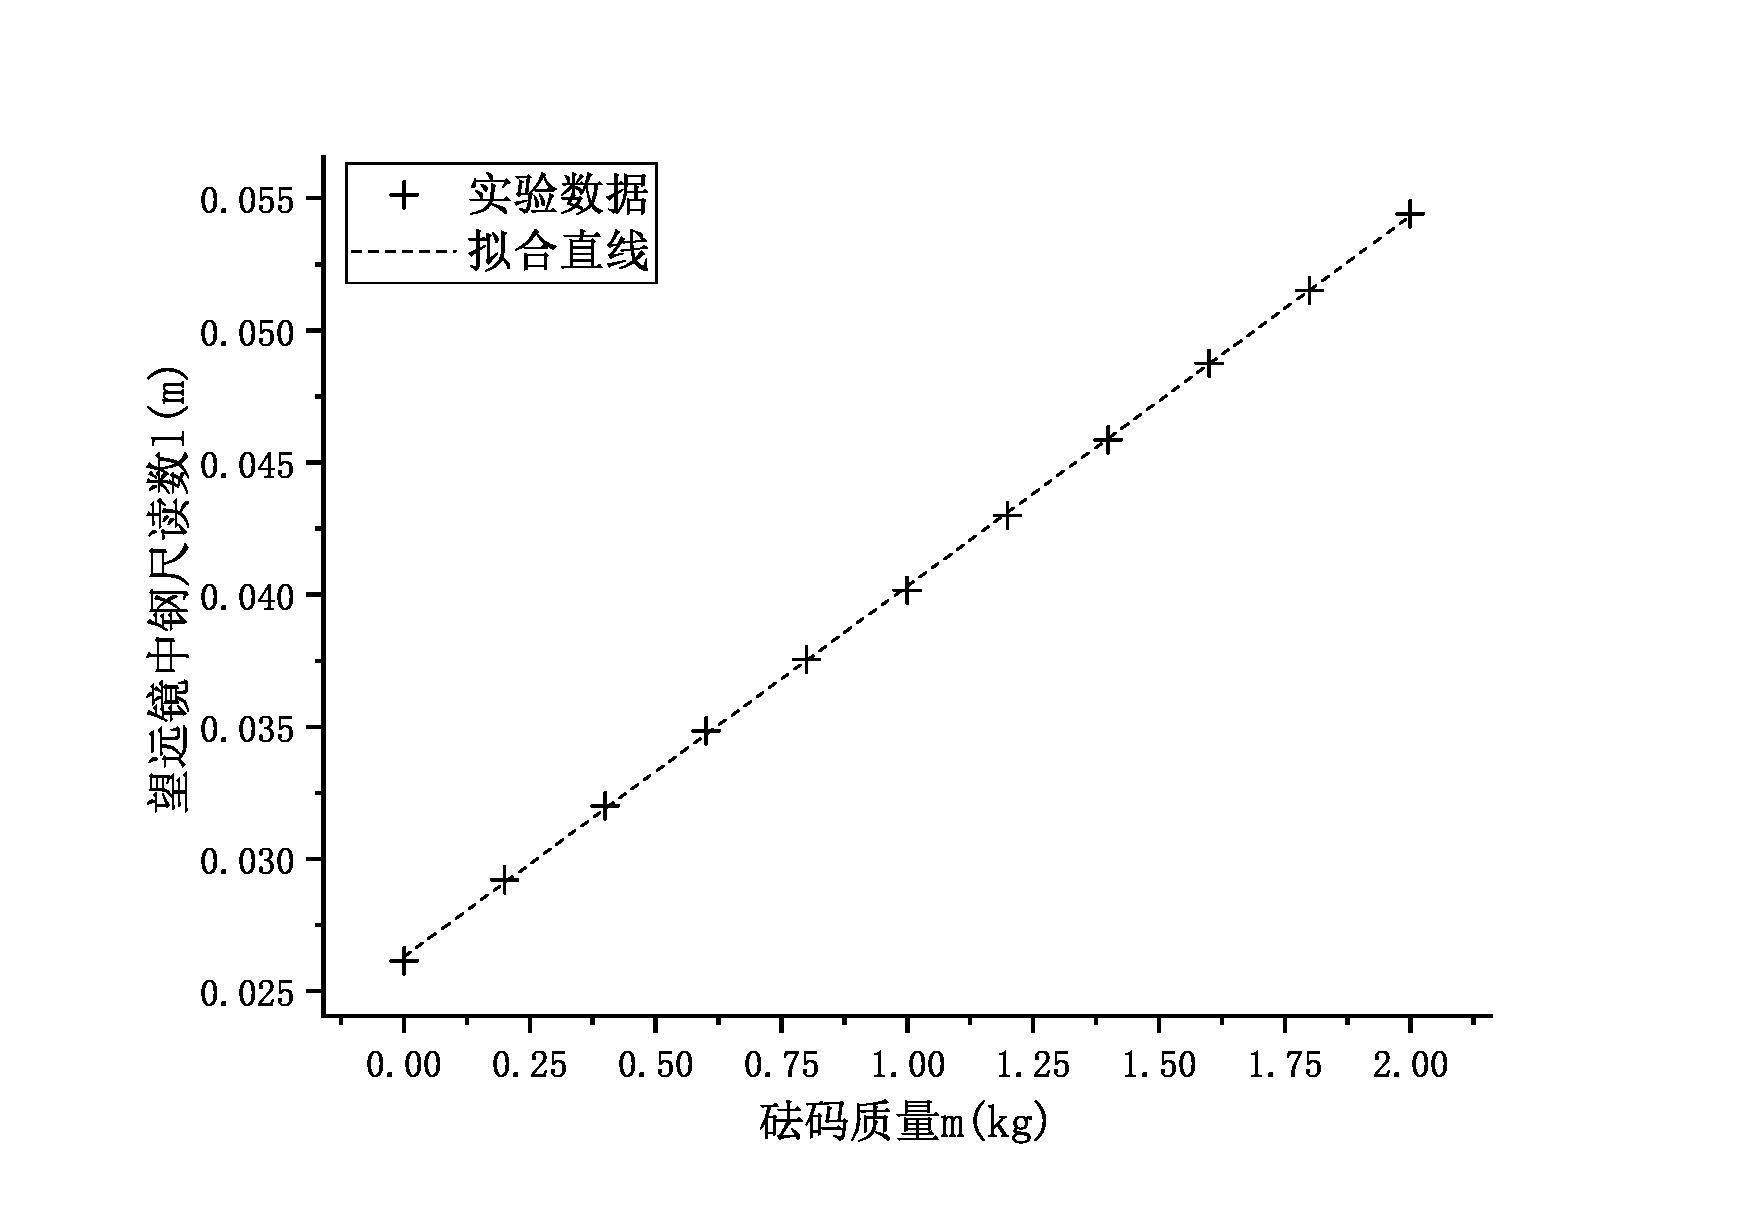
\includegraphics[scale=0.4]{2_curve.eps}
		\caption{刻度尺读数与砝码质量关系图}
	\end{figure}
	\par 
	那么我们可以计算出金属丝的杨氏模量为:
	$$
	E = \frac{8gLR}{\pi d^{2}Dk} = 1.64 \times 10^{11}\;\mathrm{Pa}
	$$
	\par 
	钢板尺的允差大约为$0.15\;\mm$,对比测量中$l$的变化(约为$3\;\cm$)来说相当小。注意这里是与CCD成像法
	测量杨氏模量相比较的,虽然显微镜刻线板的允差为$0.05\;\mm$,但是由于长度变化太小,导致相对误差很大。
	因此不经过严谨地计算,也可以看出光杠杆法测量金属的杨氏模量有着更小的不确定度。

	\subsection{梁的弯曲测定杨氏模量}
	\subsubsection{实验数据记录}
	\par 
	首先给出钢梁的相关参数:
	\begin{table}[htbp]
		\centering
		\caption{钢梁的宽度$a$与厚度$h$数据表}
		\begin{tabular}{ccccccc}
			\toprule[1.5pt]
			$a(\mm)$ & 10.149 & 10.145 & 10.120 & 10.130 & & \\
			\midrule
			$h(\mm)$ & 1.442 & 1.518 & 1.521 & 1.515 & 1.527 & 1.495\\
			\bottomrule[1.5pt]
		\end{tabular}
	\end{table}
	\par 
	从上表的数据可以看出钢梁的参数相对于钢丝来说标准差更大,从实验测量发现钢梁在靠近两端的地方测量值
	会明显偏小。同时计算出$\bar{a} = 10.136\;\mm,\;\bar{h}=1.503\;\mm$。
	\begin{table}[htbp]
		\centering
		\caption{读数显微镜读数$\lambda$与钢梁下砝码质量数据表}
		\begin{tabular}{ccccc}
			\toprule[1.5pt]
			$i$ & $m_{i}(\g)$ & $\lambda_{i}(mm)$ & $\lambda_{i}^{'}(\mm)$ & $\bar{\lambda_{i}}(\mm)$\\
			\midrule
			0 & 0      & 44.213 & 44.200 & 44.2065\\
			1 & 200.82 & 43.838 & 43.845 & 43.8415\\
			2 & 400.50 & 43.498 & 43.500 & 43.499 \\
			3 & 600.46 & 43.160 & 43.162 & 43.161 \\
			4 & 800.94 & 42.802 & 42.800 & 42.801 \\
			5 & 1000.57& 42.480 & 42.480 & 42.480 \\
			\bottomrule[1.5pt]
		\end{tabular}
	\end{table}
	\par 
	最后给出钢梁两个支点之间的距离,即有效长度$l=17.20\;\cm$。
	\subsubsection{使用最小二乘法处理数据}
	\par 
	当挠度很小时,材料的杨氏模量可以表示为:
	$$
	E = \frac{\Delta mg l^{3}}{4\Delta \lambda a h^{3}}
	$$
	\par 
	表示为方便进行线性回归的形式:
	$$
	\Delta \lambda = \frac{gl^{3}}{4Eah^{3}} \Delta {m}
	$$
	\par 
	通过最小二乘法得到$|k| = 0.00173\;\mathrm{m/kg},\;r^{2} = 0.9998$
	\begin{figure}[htbp]
		\centering
		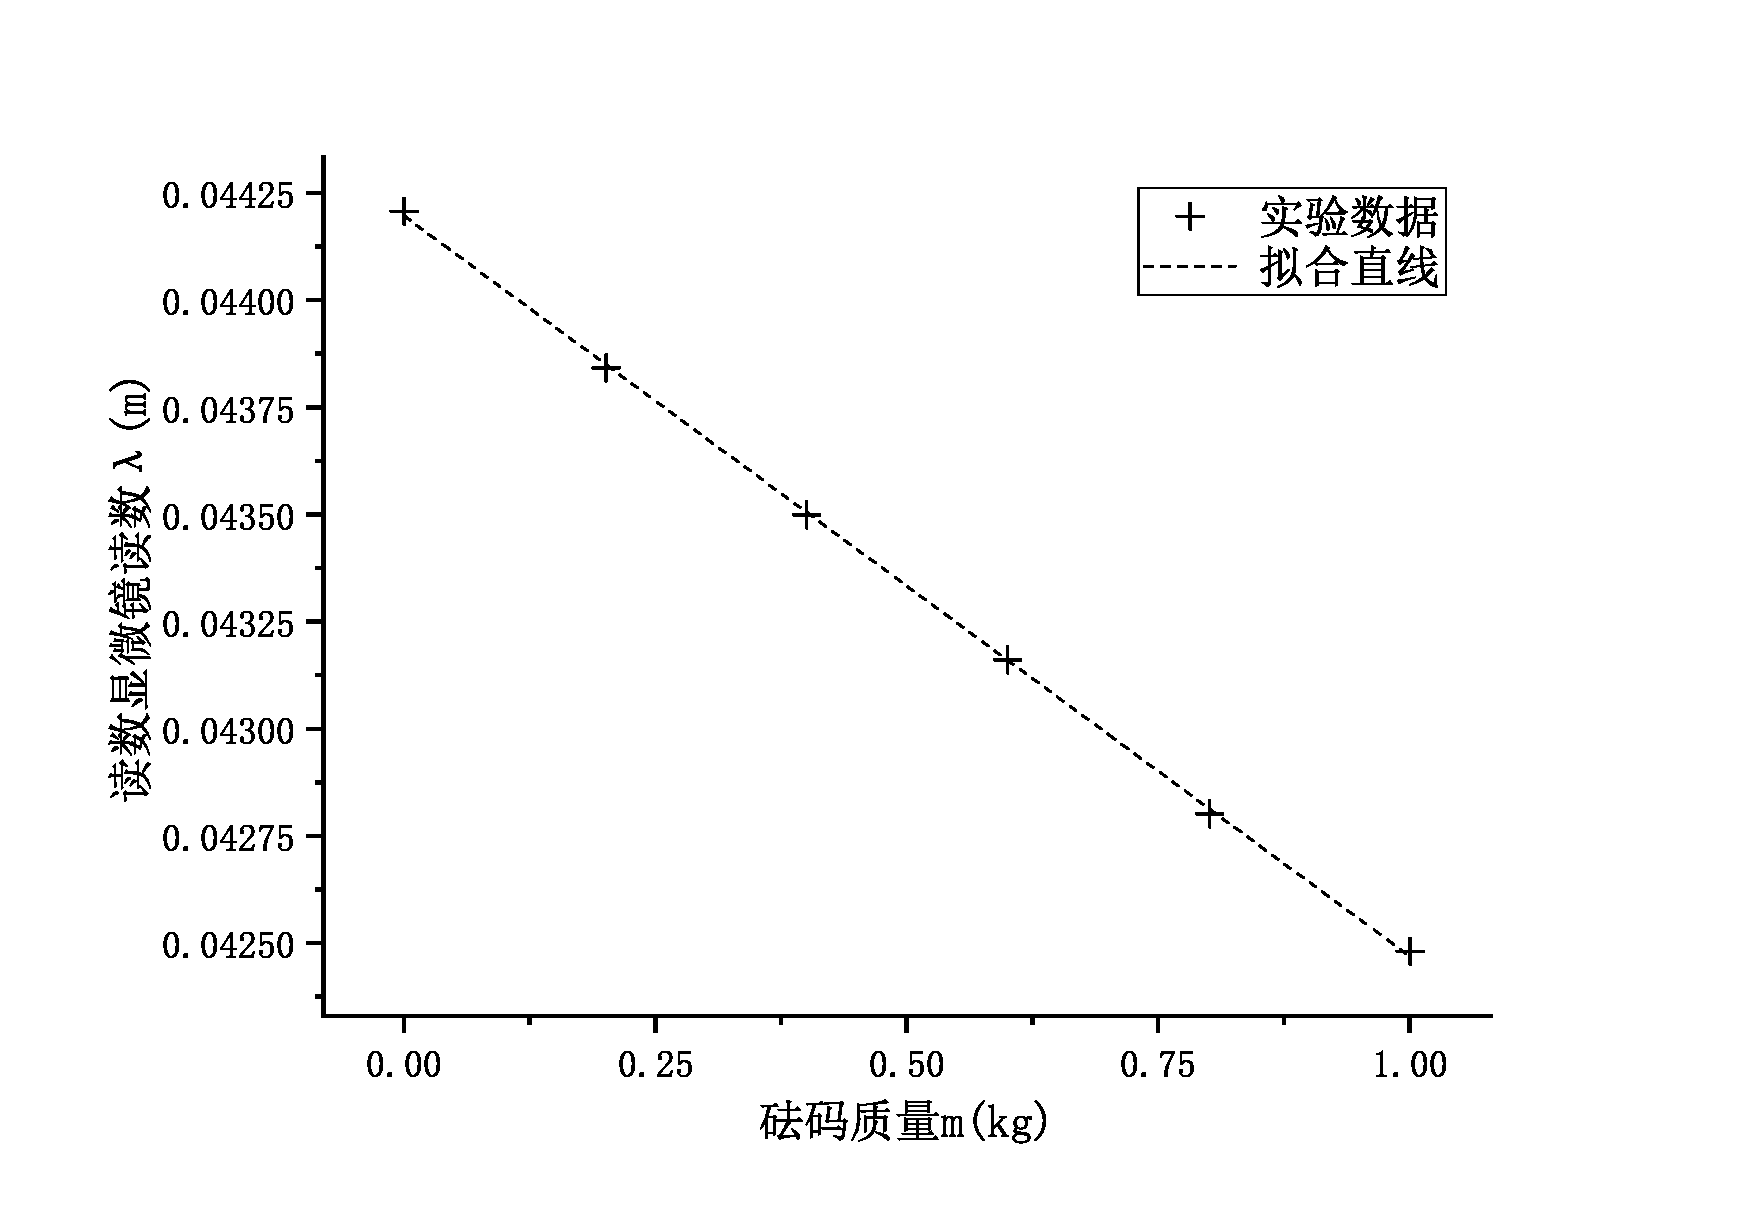
\includegraphics[scale=0.4]{3_curve.eps}
		\caption{读数显微镜读数与钢梁下砝码质量关系图}
	\end{figure}
	\par 
	由杨氏模量的表达式可以得到:
	$$
	E = \frac{gl^{3}}{4kah^{3}} = 2.09 \times 10^{11}\;\Pa
	$$
	\section{\large{分析与讨论}}
	\paragraph{实验开始时金属丝伸长量不均匀的问题}
	由于金属丝不是严格意义上的细丝,是有粗细的,因此金属丝除了可以承受
	径向的拉力之外,还可以产生一定的垂直于细丝方向的力。这就导致了
	自由悬挂的金属丝不一定是竖直的,尤其是当金属丝上有小的弯折时,
	便可以承受较大的拉力而不完全伸直。实验中使用的金属丝难免会有这样的
	弯折,所以在刚开始加入砝码时,除了金属丝自身在拉力作用下伸长之外,
	还会因为弯折部分变直而产生额外的伸长,因此,在最初加砝码时会观察到
	伸长量偏长的现象;为了尽可能消除这种现象,可以在测量开始时先在金属丝
	下方挂上一定质量的砝码,同时应该实验结束后测量金属丝的直径,因为
	使用螺旋测微器测量有可能造成金属丝的进一步弯折。
	\par 
	如果调节实验装置时竖直方向上残余了比较明显的摩擦力,那么这样产生的
	相对误差会因为砝码质量增加而减小,那么在最开始加砝码时会观察到
	伸长量偏小。
	\paragraph{金属丝直径不均匀的问题}
	在实验测量中发现,金属丝的直径在靠近两端的地方偏大,而中间部位的
	直径非常均匀。这就说明金属丝的直径不均匀并不是由于生产原因造成的,
	只有可能是使用中的某些原因导致了金属丝的直径变化。个人推测的原因是
	由于金属丝在测量、调节仪器时都会产生振动或者晃动,由于两端可以近似
	认为是固定的,在晃动的过程中靠近两端的金属会受到反复的弯折,尤其是
	固定金属丝的地方一定非常容易出现疲劳,所以这部分的金属丝很可能偏离了
	理想的圆柱形,导致螺旋测微器在测量时无法用平面“卡住”直径,从而导致
	测量出的直径数据偏大,实验中的测量结果也正是这样。\\
	\\
	\section{\large{收获与感想}}
	\par 
	这次的实验内容比较多,操作也比较繁杂,所以相比之前的实验消耗了更多的
	时间,对同学与老师的耐心都是一个不小的挑战(尤其是光杠杆用了很长时间
	才调节好的时候)。在实验时由于读数读的我眼花缭乱因此向同学吐槽说感觉
	每次的实验都像是光学实验,没想到那个同学认真地告诉我:因为光信号是最
	容易精确测量的信号呀。仔细一想,确实是这么回事,很多时候我们都是把难以
	察觉的量转化为光信号,这样不仅方便实验者观察实验现象并对实验做出调整
	也便于精确测量,这也让我想起了上周做的迈克尔逊干涉仪的实验,正是通过
	干涉条纹的变化,我们可以对很多几乎无法测量的量进行精确的测量。
	\par 
	在这次实验中我觉得最重要的除了如何测量金属丝(或者钢梁)的形边量,还有
	各种各样的长度测量值得关注。由于我们待测的长度可能处于空间中的不同位置,
	或者被测量的的物体有着各种各样的奇怪形状使得尺子并不易接近,对应的例子
	就有金属丝长度的测量与光杠杆长度的测量。在第一次测量光杠杆的长度时由于
	测量方法问题,测量的长度明显偏大,导致了计算出的杨氏模量明显偏小,在老师
	的提醒之下,才想到了精确测量光杠杆长度的方法,就是把光杠杆上的三个支点
	画在纸上,这样就可以很方便地做出垂线进而求出光杠杆的长度。这么看来,在
	很多实验细节中可能都隐藏着一些值得仔细思考的大学问。
\end{document}